\section{Resultados}

\subsection{Resultados en el conjunto de prueba}
La Tabla~\ref{tab:test} y la Fig.~\ref{fig:test} muestran el desempeño en prueba del modelo seleccionado en cada escenario. Todos los modelos que usan las variables originales o la URL completa obtienen F1 entre 0,996 y 1,000; el Random Forest con las 50 variables no comete errores en las 35.246 URLs. Quitar \texttt{URLSimilarityIndex} (A2) o las variables de la página (A3) no cambia este resultado, porque las variables de la URL se calcularon sobre la URL completa y también reflejan el prefijo y la ruta. En A1 y A2 incluso la regresión logística supera 0,999 en validación, otra señal de que el problema, tal como está planteado, es artificialmente fácil.

\begin{table}[t]
\caption{Resultados en prueba (clase positiva: phishing)}
\label{tab:test}
\centering
\setlength{\tabcolsep}{4pt}
\begin{tabular}{llcccc}
\toprule
Modelo & Entrada & P & R & F1 & AUC \\
\midrule
RF & A1: 50 variables & 1,000 & 1,000 & 1,000 & 1,000 \\
MLP & A2: 49 variables & 1,000 & 1,000 & 1,000 & 1,000 \\
MLP & A3: 21 de la URL & 1,000 & 0,995 & 0,997 & 0,999 \\
TF-IDF + RL & URL original & 1,000 & 0,993 & 0,996 & 0,999 \\
CNN & URL original & 1,000 & 0,995 & 0,997 & 0,999 \\
TF-IDF + RL & URL normalizada & 0,946 & 0,814 & 0,875 & 0,943 \\
\midrule
TF-IDF + RL & Dominio & 0,913 & 0,762 & \textbf{0,830} & 0,919 \\
CNN & Dominio & 0,952 & 0,728 & 0,825 & 0,919 \\
BiGRU & Dominio & 0,953 & 0,709 & 0,813 & 0,910 \\
XGBoost & A4: léxicas del dominio & 0,921 & 0,672 & 0,777 & 0,881 \\
\bottomrule
\multicolumn{6}{l}{\footnotesize Sobre la línea: usan atajos. Bajo la línea: solo el dominio.}
\end{tabular}
\end{table}

\begin{figure}[t]
\centering
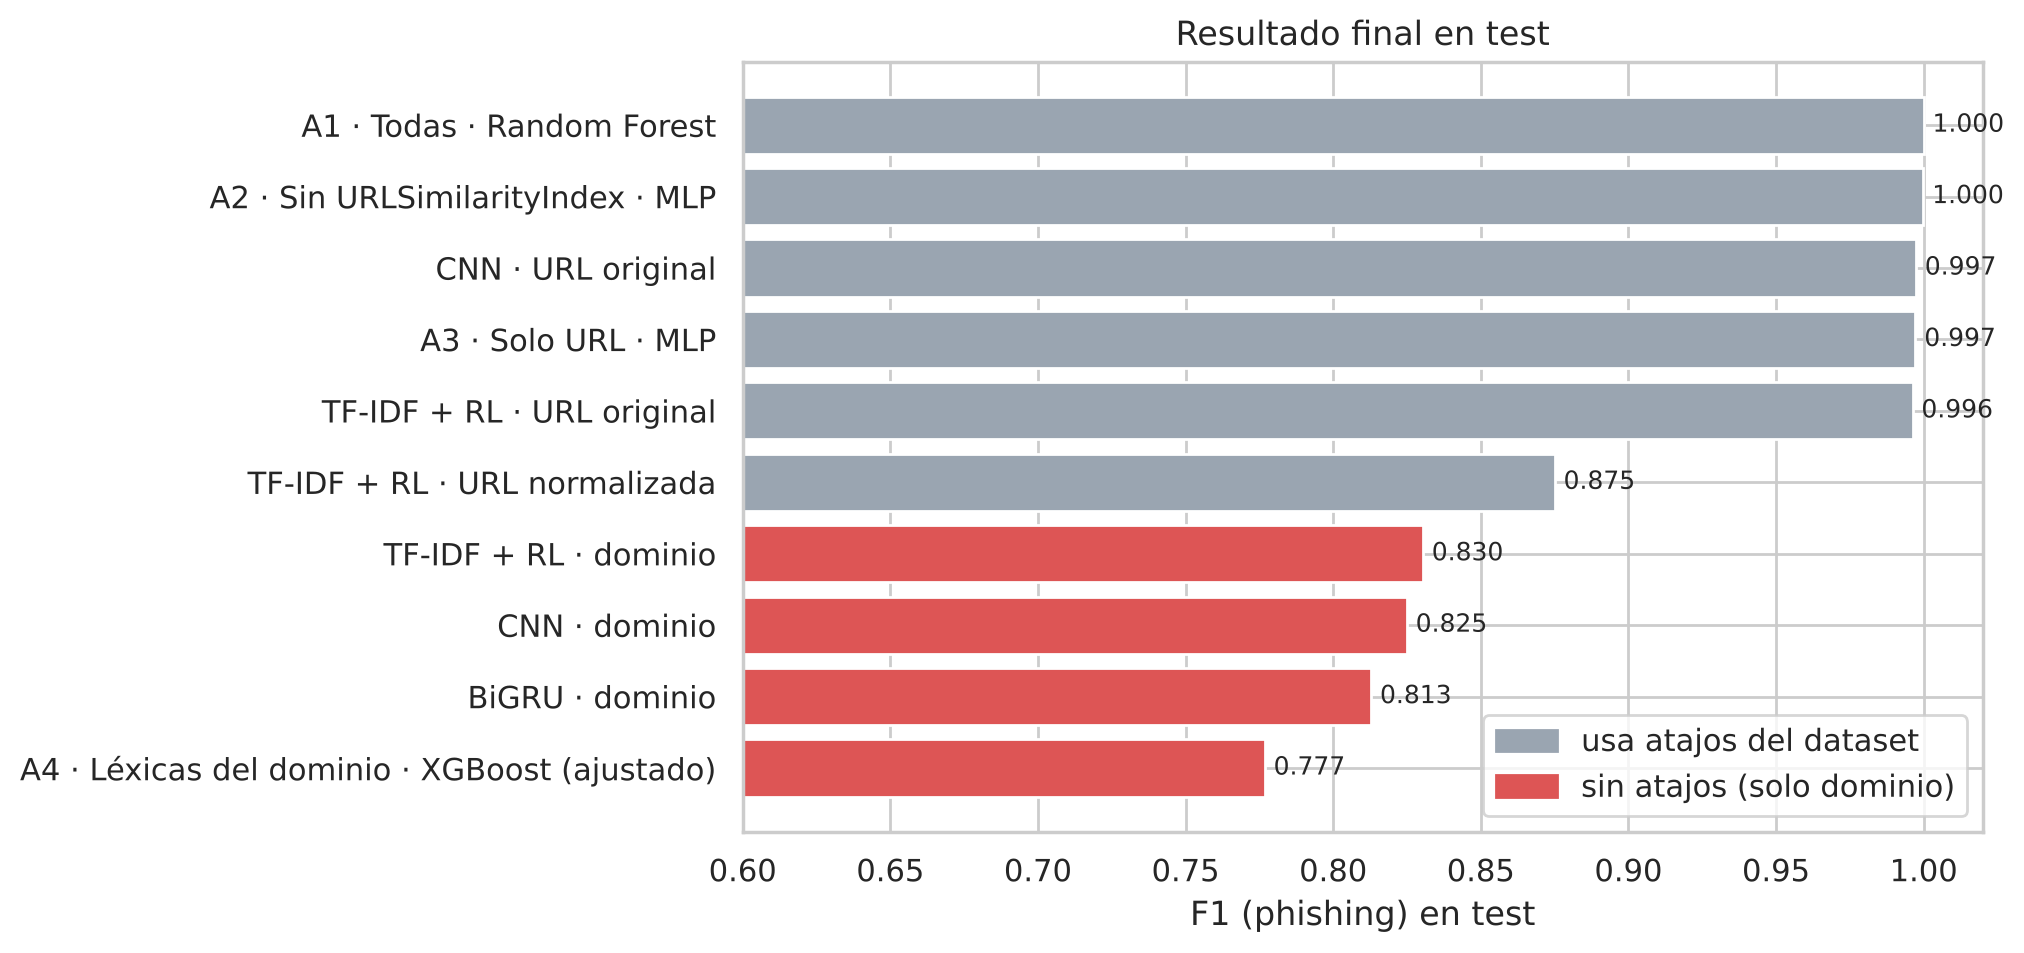
\includegraphics[width=\columnwidth]{12_resultados_test.png}
\caption{F1 en prueba. En gris, los modelos que usan atajos; en rojo, los que solo ven el dominio.}
\label{fig:test}
\end{figure}

Sin atajos, el desempeño cae a F1 $\approx$ 0,83. Entre los modelos de dominio, TF-IDF con regresión logística (0,830) y la CNN de caracteres (0,825) quedan prácticamente empatados, con el mismo ROC-AUC (0,919); la CNN es más precisa (0,952 frente a 0,913) y TF-IDF detecta más phishing (\emph{recall} 0,762 frente a 0,728). La BiGRU queda algo por debajo (0,813) y tarda más del doble en entrenarse en CPU. Los tres modelos de texto superan en 4 a 5 puntos de F1 al mejor modelo con variables léxicas hechas a mano (XGBoost, 0,777), cuyo ajuste de hiperparámetros aportó cerca de un punto de F1 en validación. Con textos cortos como un dominio, los n-gramas de caracteres ya capturan gran parte de la información disponible, por lo que la red neuronal no supera con claridad a una línea base bien construida.

\begin{figure*}[t]
\centering
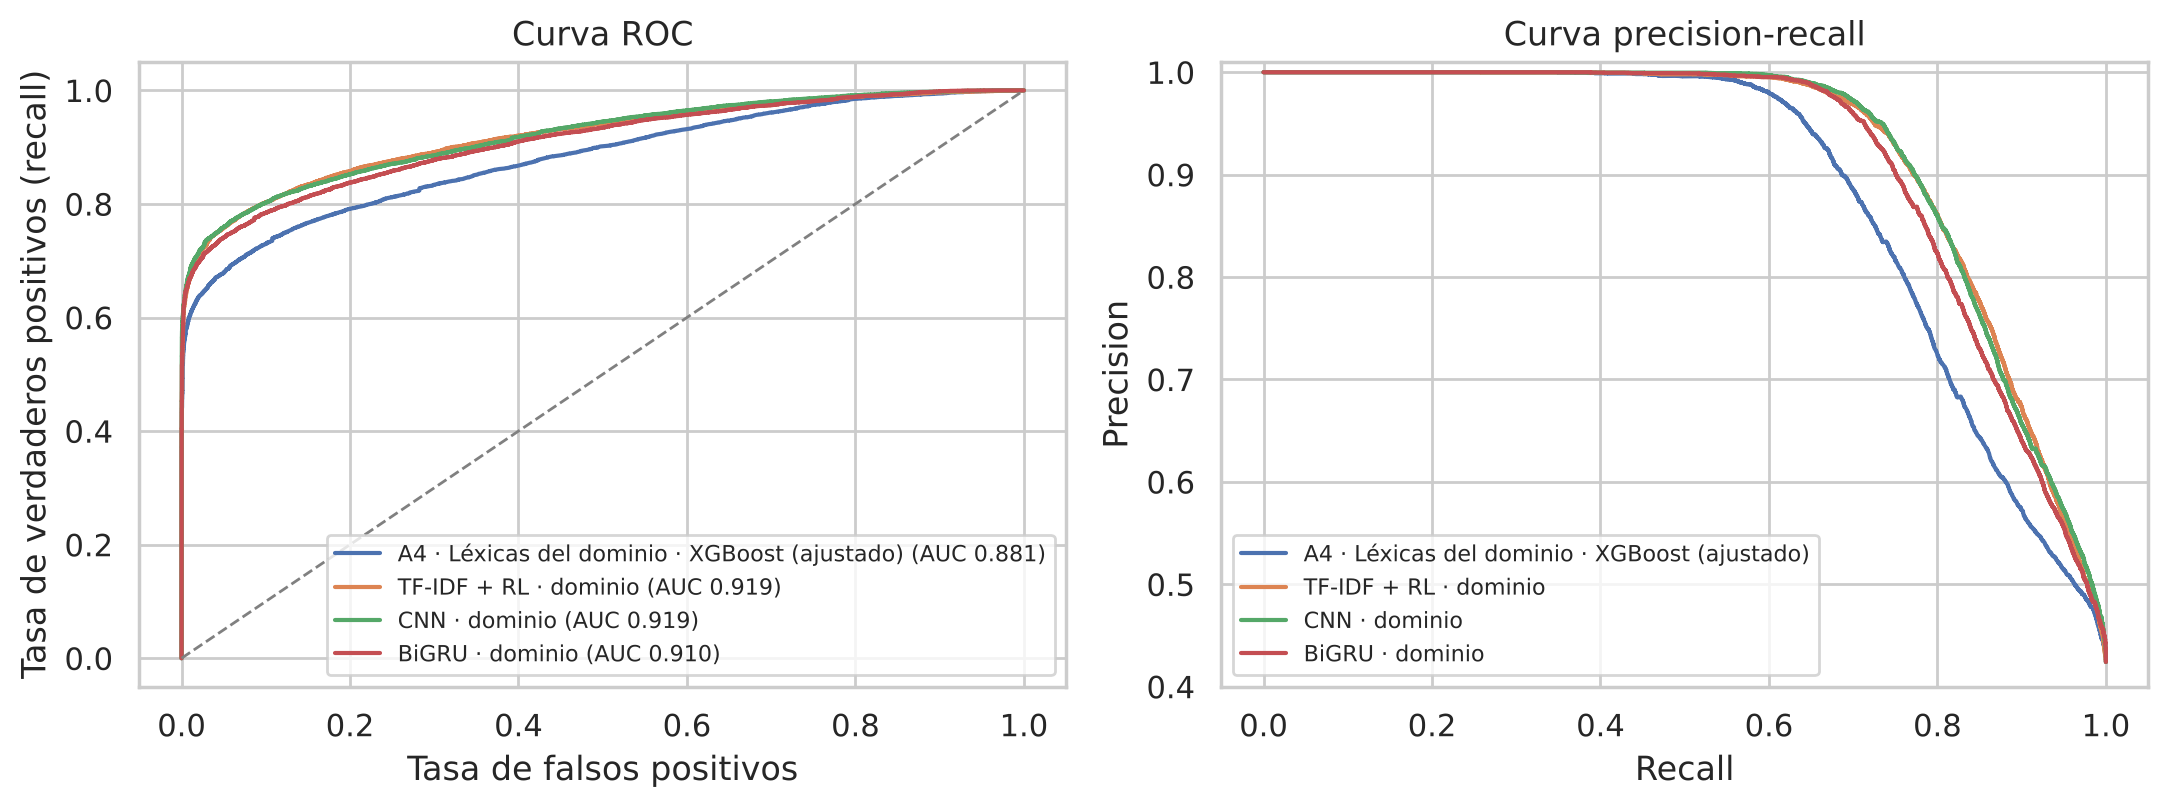
\includegraphics[width=0.8\textwidth]{14_roc_pr_dominio.png}
\caption{Curvas ROC y precisión-\emph{recall} en prueba de los modelos que solo ven el dominio.}
\label{fig:roc}
\end{figure*}

La Fig.~\ref{fig:roc} muestra que las curvas de TF-IDF y de la CNN prácticamente se superponen, y que ambas dominan a XGBoost con variables léxicas en todo el rango de umbrales.

\subsection{Interpretación}
Con SHAP, el modelo de A2 se apoya sobre todo en variables de la página (líneas de código, referencias propias y externas) y en \texttt{IsHTTPS}, que reflejan el modo de recolección. En A4, las variables más influyentes son la cantidad de puntos del dominio, su largo, los dígitos y el largo del TLD. Los n-gramas con mayor peso hacia phishing en el modelo TF-IDF corresponden a TLDs gratuitos o de bajo costo (\texttt{.cf}, \texttt{.ga}, \texttt{.ml}, \texttt{.top}); hacia legítima, a \texttt{.gov}, \texttt{.edu}, \texttt{.mil} y TLDs de países.

\subsection{Prueba con URLs fuera del dataset}
Para comprobar el efecto de los atajos se clasificaron URLs escritas a mano (Tabla~\ref{tab:manual}). La CNN entrenada con la URL original asigna probabilidad 1,000 de phishing a cinco URLs legítimas reales, solo porque tienen ruta o subdominio. La CNN de dominio clasifica bien \texttt{github.com}, pero deja \texttt{google.com} y \texttt{es.wikipedia.org} cerca del umbral y marca \texttt{mail.google.com} como phishing.

\begin{table}[t]
\caption{Probabilidad de phishing en URLs escritas a mano}
\label{tab:manual}
\centering
\resizebox{\columnwidth}{!}{%
\begin{tabular}{lcc}
\toprule
URL & CNN URL & CNN dominio \\
\midrule
\multicolumn{3}{l}{\emph{Legítimas}} \\
\texttt{https://www.google.com/maps} & 1,000 & 0,527 \\
\texttt{https://es.wikipedia.org/wiki/Phishing} & 1,000 & 0,592 \\
\texttt{https://github.com/54isaac09} & 1,000 & 0,320 \\
\texttt{https://www.ubiobio.cl/w/} & 1,000 & 0,604 \\
\texttt{https://mail.google.com/mail/u/0/} & 1,000 & 0,998 \\
\multicolumn{3}{l}{\emph{Phishing inventadas}} \\
\texttt{http://secure-login-verify-account.xyz/signin} & 1,000 & 1,000 \\
\texttt{http://192.168.10.5/bank/login.php} & 1,000 & 1,000 \\
\bottomrule
\end{tabular}}
\end{table}

Esto revela un sesgo residual en el dominio: solo el 4~\% de los dominios legítimos tiene subdominio (además de \texttt{www}), frente al 55~\% de los de phishing, y hay 921 URLs de phishing con ``google'' en el dominio (por ejemplo, formularios en \texttt{docs.google.com}) frente a 12 legítimas. Por lo tanto, el F1 de 0,83 también es optimista respecto de un escenario real.

\subsection{Umbral y errores}
Con el umbral por defecto (0,5) la CNN de dominio deja pasar 4.068 URLs de phishing. Un umbral de 0,16, elegido en validación para alcanzar 90~\% de \emph{recall}, logra 0,894 de \emph{recall} en prueba, pero la precisión baja a 0,669. Los phishing no detectados se parecen a dominios comunes: el 40,9~\% de los que terminan en \texttt{.com} se escapa, frente al 17,2~\% del resto, y solo el 3,9~\% de los que contienen dígitos.

\section{Conclusiones}

Se implementó y evaluó una rutina completa de detección de URLs de phishing con siete modelos de Machine Learning y Deep Learning sobre PhiUSIIL. Con las variables originales o la URL completa, todos los modelos alcanzan F1 entre 0,996 y 1,000, en línea con lo reportado para este dataset. Sin embargo, el análisis exploratorio mostró que este desempeño se explica por tres atajos: las URLs legítimas siempre comienzan con \texttt{https://www.}, nunca tienen ruta y siempre tienen \texttt{URLSimilarityIndex} = 100. Un modelo entrenado con la URL original clasifica como phishing cualquier URL legítima con ruta, por lo que su exactitud no se trasladaría a un uso real.

Al eliminar los atajos y usar solo el dominio, el mejor F1 en prueba fue 0,830 (TF-IDF con regresión logística), seguido de cerca por la CNN de caracteres (0,825), que fue la más precisa. Los modelos que aprenden de los caracteres superan a las variables léxicas diseñadas a mano.

Las principales limitaciones son el uso de un solo dataset, el sesgo residual de los dominios legítimos (sin subdominios) y la imposibilidad de distinguir, solo con el dominio, el phishing alojado en servicios legítimos. Como trabajo futuro se propone evaluar los modelos con otra fuente de URLs, construir un conjunto con URLs legítimas que incluyan rutas y subdominios, combinar dominio y ruta en ese conjunto y explicar las predicciones de la CNN.
